\chapter{Ranking}
We have chosen a \textbf{lnc.ltc} (using SMART notation) ranker, where the latter refers to the method applied to the query.
We chose this option because we used the approach for the course exercises - so it supplied us with some prior knowledge of how to apply the method and some good test cases.
In the table below the other variants are shown:

\begin{center}
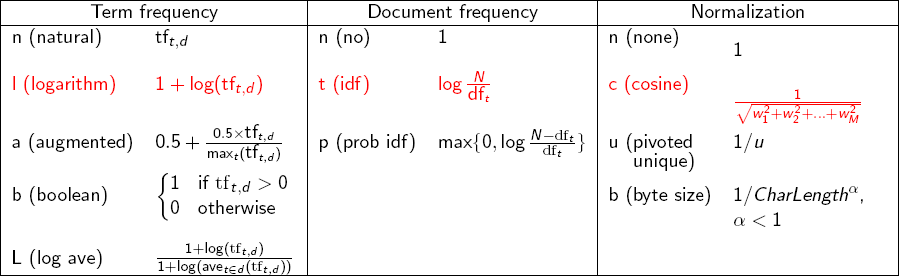
\includegraphics[width=\linewidth]{graphics/rankingmethods}
\end{center}

Below we will try and describe the process - the input are all the documents in the index:
\begin{enumerate}
\item A table with term frequencies is calculated
\item A table with document frequencies is calculated
\item The two tables get combined by multiplying the frequencies to create a weigthed table
\item The weighted is then normalized.
\item If there is an input query it will get calculated just the way a document gets calculated.
\item Then the distance between the normalized vectors between the query and all the documents is calculated.
\item The document closest is the best hit in the search engine.
\end{enumerate}
